\documentclass[10pt]{article}
\usepackage[utf8]{inputenc}
\usepackage[activeacute,spanish]{babel}
\usepackage[left=1.5cm,top=1.5cm,right=1.5cm, bottom=1.5cm,letterpaper, includeheadfoot]{geometry}

\usepackage{amssymb, amsmath, amsthm}
\usepackage{graphicx}
\usepackage{hyperref}
\usepackage{lmodern,url}
\usepackage{paralist} %util para listas compactas
\usepackage{xcolor}
\usepackage{bbm}
\usepackage{mathrsfs}
\usepackage{bbm}

%========PAQUETES AGREGADOS===========
%Pseudocodigo
\usepackage{pseudocode}
\usepackage[portuguese, boxruled]{algorithm2e}
\usepackage{wrapfig}
\usepackage{multicol}
\usepackage{graphicx}
\usepackage{caption}
\usepackage{subcaption}
%\captionsetup[table]{labelformat=empty}
\captionsetup[subfigure]{labelformat=empty}
\usepackage{cancel}
\usepackage{tikz}
\def\checkmark{\tikz\fill[scale=0.4](0,.35) -- (.25,0) -- (1,.7) -- (.25,.15) -- cycle;} 
%====================================

\usepackage{fancyhdr}
\pagestyle{fancy}
\fancypagestyle{plain}{%
\fancyhf{}
\lhead{\footnotesize\itshape\bfseries\rightmark}
\rhead{\footnotesize\itshape\bfseries\leftmark}
}


% macros
\newcommand{\Q}{\mathbb Q}
\newcommand{\R}{\mathbb R}
\newcommand{\N}{\mathbb N}
\newcommand{\Z}{\mathbb Z}
\newcommand{\C}{\mathbb C}
\newcommand{\BigO}{\mathcal{O}}
%Teoremas, Lemas, etc.
\theoremstyle{plain}
\newtheorem{teo}{Teorema}
\newtheorem{lem}{Lema}
\newtheorem{prop}{Proposición}
\newtheorem{cor}{Corolario}
\newtheorem{obs}{Observación}
\newtheorem{ej}{Ejemplo}
\renewcommand{\qedsymbol}{\rule{0.7em}{0.7em}}
\renewenvironment{proof}{{\bfseries \noindent Demostración}}{ \qed \\}


\theoremstyle{definition}
\newtheorem{defi}{Definición}
% fin macros


\newcommand{\catnum}{22} %numero de catedra
\newcommand{\fecha}{29 de Noviembre 2016 }

%%%%%%%%%%%%%%%%%%

%Macros para este documento
\newcommand{\cin}{\operatorname{cint}}



\begin{document}
%Encabezado
\fancyhead[L]{Facultad de Ciencias Físicas y Matemáticas}
\fancyhead[R]{Universidad de Chile}
\vspace*{-1.2 cm}
\begin{minipage}{0.6\textwidth}
\begin{flushleft}
\hspace*{-0.5cm}\textbf{MA3402-1 Estadística. Primavera 2016}\\
\hspace*{-0.5cm}\textbf{Profesor:} Raul Gouet\\
\hspace*{-0.5cm}\textbf{Escriba:} Manuel Cáceres\\
\hspace*{-0.5cm}\textbf{Fecha:} \fecha
\end{flushleft}
\end{minipage}
\begin{minipage}{0.36\textwidth}
\begin{flushright}

\includegraphics[scale=0.3]{imagenes/fcfm_dcc}
\end{flushright}
\end{minipage}
\bigskip
%Fin encabezado

\begin{center}
\LARGE\textbf{Clase \catnum}
\end{center}
Recién vimos el teorema Gauss-Markov, según el cual, bajo las hipótesis ``clásicas'', el EMC de $\beta$ es el mejor entre los lineales insesgados.\\

Hipótesis clásicas: $X$ de rango completo, $\epsilon$ con $\mathbb{E}(\epsilon) = 0$, $\mathbb{E}(\epsilon\epsilon')=\sigma^2I$.\\

$\hat{\beta} = (X'X)^{-1}X'Y$ es el EMC.\\

Si consideramos la función de $\beta$, $\phi = a'\beta$. El estimador $\hat{\phi} = a'\hat{\beta}$ es óptimo, en la clase de estimadores insesgados del tipo $\tilde{\phi} = b'Y$.\\

\section{Estimación de $\sigma^2$}
$\sigma^2$ (la varianza de los errores) es un parámetro más del modelo. Digamos que $\theta = (\beta, \sigma) \in \Theta = \mathbb{R}\times(0,\infty)$.\\

Para estimar $\sigma$ vamos a recurrir a los residuos $\hat{\epsilon}$ del modelo
\begin{center}
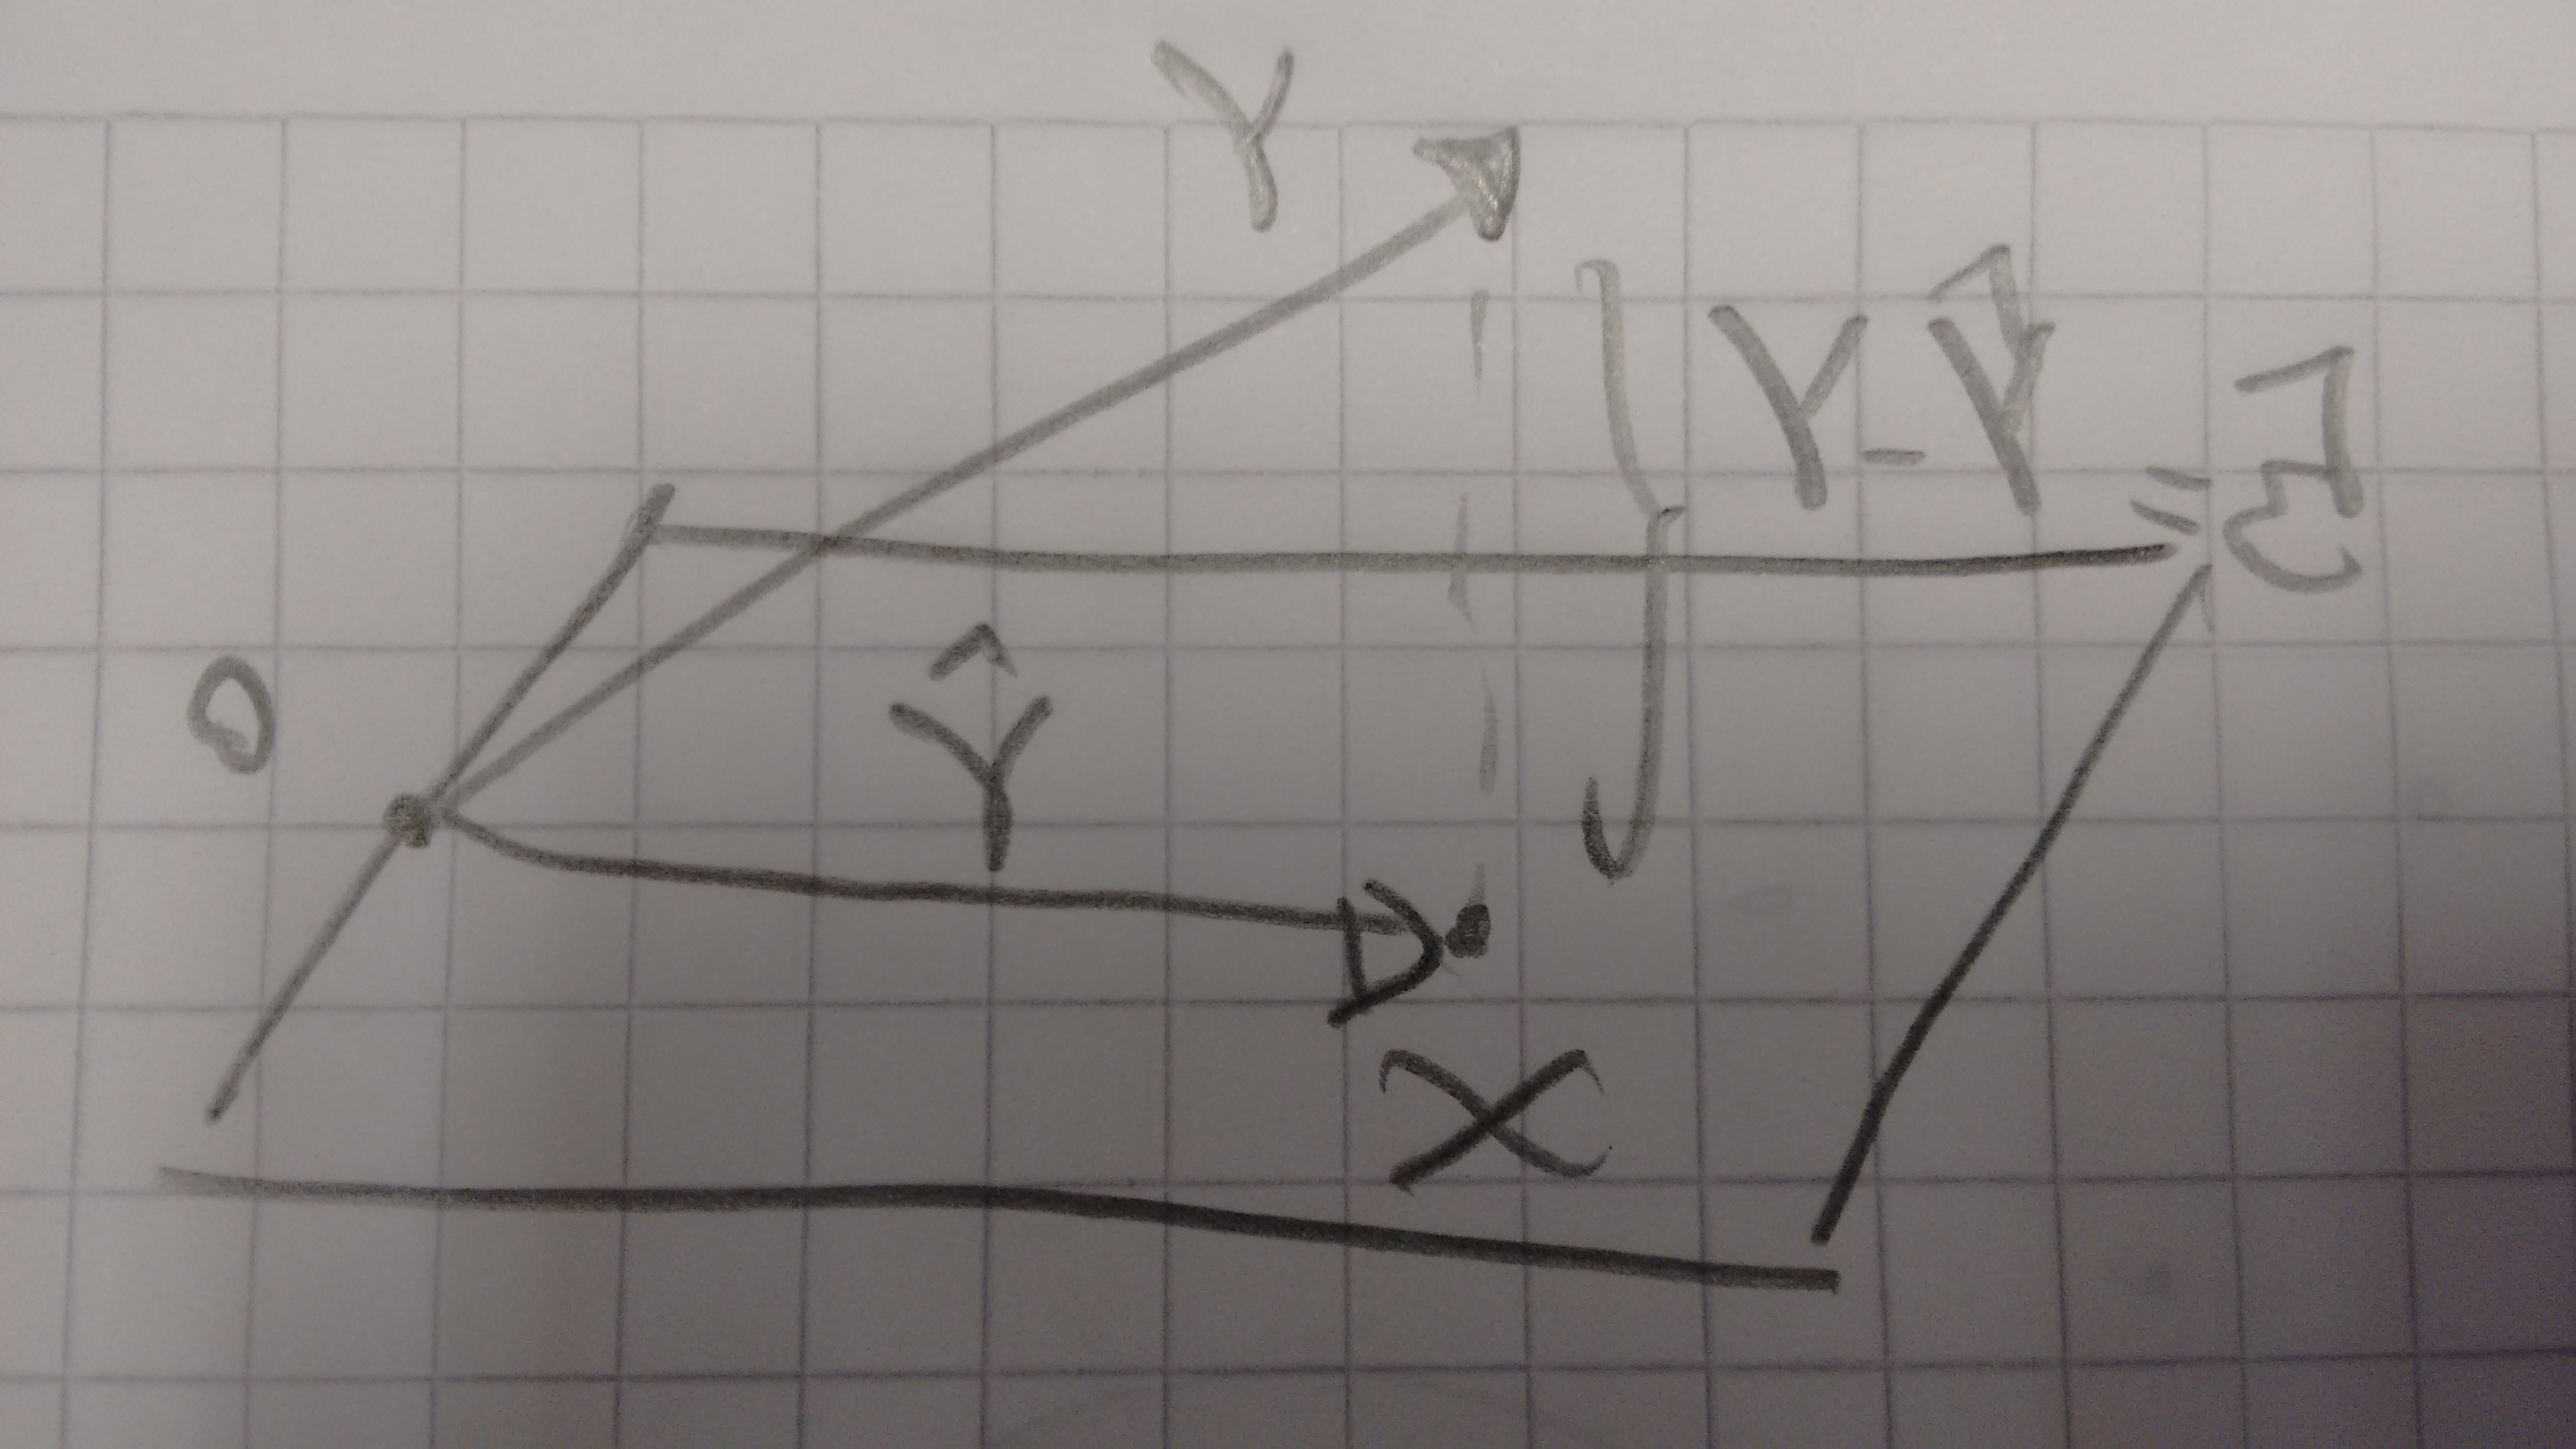
\includegraphics[scale=0.1]{imagenes/proyeccion.jpg}
\end{center}

$\hat{\epsilon} = Y - \hat{Y} = $ la parte no ``explicada'' por las variables $X$.\\

Recordemos que $Y$ tiene $\mathbb{E}(Y) = X\beta \in <X>$.\\

Notemos que $\mathbb{E}(\hat{\epsilon}) = 0$. Ahora calculemos la esperanza de $||\hat{\epsilon}||^2 = (Y-X\hat{\beta})'(Y-X\hat{\beta})$. Notemos que
\begin{align*}
\hat{\epsilon} &= Y -X \hat{\beta}\\
&= \underbrace{(I-X(X'X)^{-1}X')}_{proyector\ en\ <X>^{\perp}}Y\\
&= QY\\
&= Q(X\beta + \epsilon)\\
&= Q\epsilon
\end{align*}
Entonces
\begin{align*}
\mathbb{E}(||\hat{\epsilon}||^2) &= \mathbb{E}(\hat{\epsilon}'\hat{\epsilon})\\
&= \mathbb{E}((Q\epsilon)'Q\epsilon)\\
&= \mathbb{E}(\epsilon'Q'Q\epsilon)\\
&= \mathbb{E}(\epsilon'Q\epsilon)\\
&= \mathbb{E}(tr(\epsilon'Q\epsilon))\\
&= \mathbb{E}(tr(\epsilon\epsilon'Q))\\
&= tr(\mathbb{E}(\epsilon\epsilon'Q))\\
&= tr(\underbrace{\mathbb{E}(\epsilon\epsilon')}_{\sigma^2I}Q)\\
&= \sigma^2 tr(Q)\\
&= \sigma^2 (n-k)
\end{align*}
Concluímos que $\hat{\sigma}^2 = \frac{1}{n-k} ||\hat{\epsilon}||^2$ es estimador insesgado para $\sigma^2$ en el modelo de rango completo clásico.\\

Recordemos el problema de estimación de $\mu = \mathbb{E}(X_{i})$ y $\sigma^2 = Var(X_{i})$ en una muestra iid $X_{1},\ldots, X_{n}$ de una distribución cualquiera.\\

Esto se puede escribir en el lenguaje de los modelos lineales
\begin{align*}
X_{i} &= \mu + \epsilon_{i}, \forall i = 1\ldots n
\end{align*}
Definimos el modelo lineal con $Y = \begin{bmatrix}
           X_{1} \\
           X_{2} \\
           \vdots \\
           X_{n}
         \end{bmatrix}, \beta = \mu, X = \begin{bmatrix}
           1 \\
           1 \\
           \vdots \\
           1
         \end{bmatrix}$
\begin{align*}
\underbrace{Y}_{n\times 1}=X\underbrace{\beta}_{1\times 1} +\epsilon &\quad \hat{\mu} = \hat{\beta} = \underbrace{(X'X)^{-1}}_{\frac{1}{n}}\underbrace{X'Y}_{\sum_{i=1}^{n}X_{i}} = \bar{X}\\
k = 1 &\quad \hat{\sigma}^2 = \frac{1}{n-1} ||\hat{\epsilon}||^2\\
\hat{\epsilon} = \begin{bmatrix}
           X_{1} -\hat{X}\\
           X_{2} -\hat{X}\\
           \vdots \\
           X_{n} -\hat{X}
         \end{bmatrix} &= Y - X\hat{\beta} = \begin{bmatrix}
           X_{1} \\
           X_{2} \\
           \vdots \\
           X_{n}
         \end{bmatrix} - \bar{X} \begin{bmatrix}
           1 \\
           1 \\
           \vdots \\
           1
         \end{bmatrix}\\
||\epsilon||^2 = \sum_{i=1}^{n} (X_{i}-\bar{X})^2 &\Rightarrow \hat{\sigma}^2 = \frac{1}{n-1}\sum (X_{i}-\bar{X})^2
\end{align*}

\section{Calidad del Modelo}
La idea es cuantificar en uno o varios índices (reales) que tan bueno es el modelo.\\

Es decir, que tan bien se ajusta a los datos o que tan bien explica la variabilidad de los datos.
\begin{center}
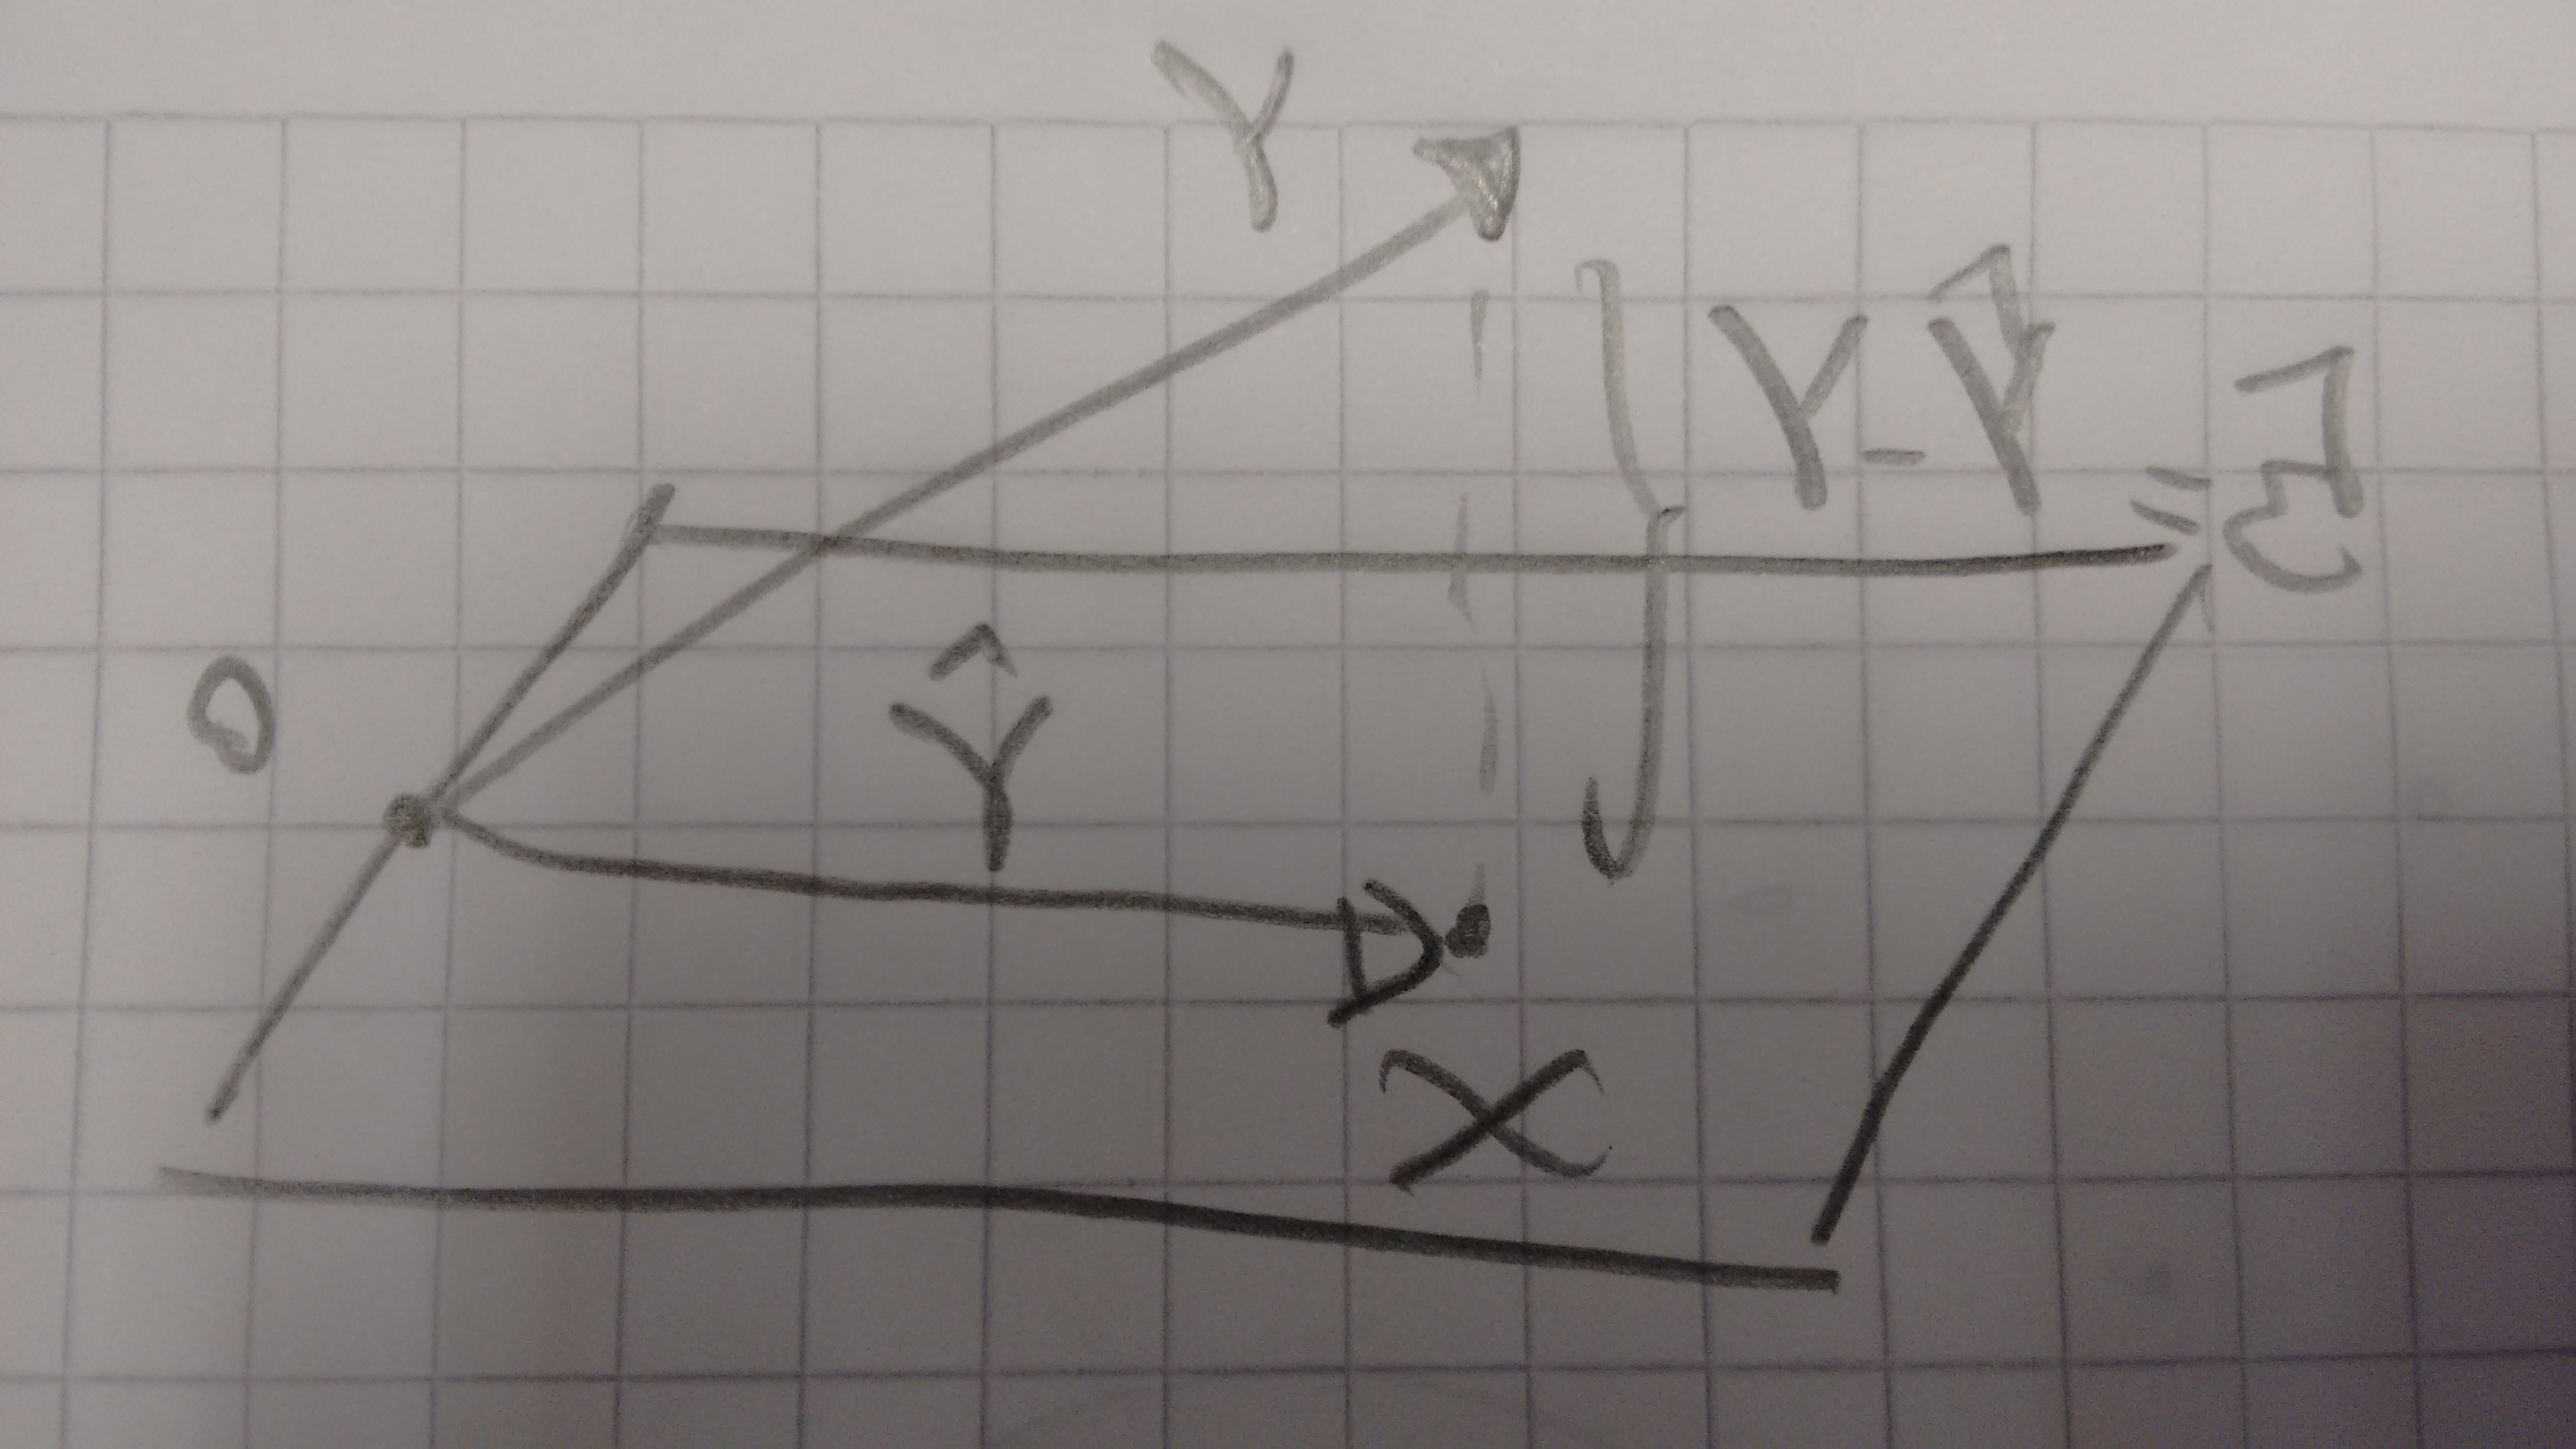
\includegraphics[scale=0.1]{imagenes/proyeccion.jpg}
\end{center}
Mientras más pequeño $||\epsilon||^2$, mejor el ajuste.\\

Se define el coeficiente $r^2$ de correlación múltiple como $cos^2$ del ángulo entre $Y$ y $<X>$
\begin{align*}
r^2=cos^2 &= \frac{||\hat{Y}||^2}{||Y||^2}\\
&= 1-\frac{||\hat{\epsilon}||^2}{||Y||^2}\\
&= \frac{<Y,\hat{Y}>^2}{||Y||^2||\hat{Y}||^2}
\end{align*}
\subsection{Interpretación:}
\begin{itemize}
\item $r^2 \approx 0 \Rightarrow$ Mal ajuste lineal
\item $r^2 \approx 1 \Rightarrow$ Buen ajuste lineal
\end{itemize}

\section{Hipótesis de Normalidad}
Aquí se supone que los $\epsilon_{i}$ son variables aleatorias normales, con $\mathbb{E}(\epsilon_{i}) = 0, \mathbb{V}(\epsilon_{i}) = \sigma^2$, es decir, $\epsilon_{i} \sim N(0,\sigma^2), i = 1\ldots n$. Ya tenemos como hipótesis $\mathbb{E}(\epsilon\epsilon') = \sigma^2I$, es decir $cov(\epsilon_{i},\epsilon_{j})=0, i\not = j$.\\

La hipótesis en definitiva es: el vector $\epsilon$ es un vector gaussiano con $\mathbb{E}(\epsilon) = 0 (vector)$ y matriz de $cov (\sigma^2I)$.\\

Recordemos la normal multivariada. Diremos que un vector $ \begin{bmatrix}
           X_{1} \\
           X_{2} \\
           \vdots \\
           X_{n}
         \end{bmatrix}$ tiene ley normal o gaussiana multivariada con esperanza $\mu \in \mathbb{R}^n$ y matriz de cov $\Sigma$ matriz de $n\times n$ definida positiva si $X$ tiene densidad
\begin{align*}
f(x) = \frac{1}{(2\pi)^{n/2}\sqrt{|\Sigma|}}e^{-\frac{1}{2}(x-\mu)'\Sigma^{-1}(x-\mu)}
\end{align*}

\subsection{Propiedades fundamentales}
\begin{itemize}
\item Si $X \sim NM(\mu, \Sigma)$ (normal multivariada), entonces todo subvector $X_{1}$ de $X$ tiene también normal con $X_{1} \sim NM(\mu_{1},\sum_{11})$.\\
\begin{align*}
X= \begin{bmatrix}
X_{1}\\ X_{2}
\end{bmatrix}\\
X_{1}\sim \mu_{1},\Sigma_{1}\quad X_{2}\sim \mu_{2},\Sigma_{2}
\end{align*}
Toda transformación lineal afín, es normal. Es decir, $Y=AX+\nu \sim NM(A\mu + \nu, A\Sigma A')$.\\

Veamos que pasa en el modelo lineal.\\
Tenemos $\epsilon \sim NM(0, \sigma^2I)$, lo cual implica que los $\epsilon_{i}$ son iid $N(0,\sigma^2)$.\\
Por otra parte, como $Y = X\beta + \epsilon$, entonces $Y \sim NM(X\beta, \sigma^{-2}I)$, $\hat{\beta} (X'X)^{-1}X'Y$.\\

Por lo tanto, $\hat{\beta} \sim NM(\beta, \sigma^2(X'X)^{-1})$.\\

Con esto podemos definir por ejemplo, intervalos de confianza.Hay más!.\\
Gracias a la normalidad se demuestra que $\hat{\beta}$ es EIVUM.\\

Aquí tenemos que simplemente notar que cada $\hat{\beta}_{i}$ tiene ley normal, $\hat{\beta}_{i} \sim N(\beta_{i}, \sigma c_{ii}), C = (c_{ij}) = (X'X)^{-1}$.\\

Podemos usar el método del pivote $\frac{\hat{\beta}_{i} - \beta_{i}}{\sigma\sqrt{c_{ii}}}$, para definir un intervalo de $\beta_{i}$, siempre que $\sigma^2$ sea conocido, si $\sigma$ es deconocido se reemplaza por $\hat{\sigma}^2 = \frac{1}{n-k} ||\hat{\epsilon}||^2$ y ocurre que $\frac{||\hat{\epsilon}||^2}{\sigma^2}$ tiene ley $\chi^2 (n-k)$ y es independiente de $\hat{\beta} - \beta$.\\

Así se construye una $t$ de student con $n-k$ grados de libertad.
\end{itemize}
\end{document}
